%! Author = Len Washington III
%! Date = 11/01/2023

% Preamble
\documentclass[title={Nov 01, 2023 Notes}]{math252notes}

% Document
\begin{document}

\setcounter{chapter}{2}
\chapter{Modeling using DE}\label{ch:modeling-using-de}
%<*Section-3.3>
\newcommand{\arrownotation}[1]{\rightarrow^{#1}\rightarrow}
\setcounter{section}{2}
\section{Applications: Modelling with a System of Linear DEs}\label{sec:applications:-modelling-with-a-system-of-linear-des}

\begin{equation*}
\begin{aligned}
	x_{1}'' + 3x_{1}' + x_{2}'' - 5x_{2} &= e^{t}\\
	x_{1}'' - 4x_{2}'' + 6x_{2}'		 &= \sin t
\end{aligned}
\end{equation*}

Two unknown functions $x_{1}(t)$ and $x_{2}(t)$. We learn methods to solve such systems in \hyperref[sec:nonhomogeneous-linear-de-with-constant-coefficients]{4.4} and 7.6.

There is usually a sequence of isotopes the initial isotope transforms through. Suppose we have Decay Series of the form \[ X\rightarrow Y\rightarrow Z \ (\mbox{ where } X \mbox{ is a stable isotope})\]

The decay rates $X\rightarrow Y$ and $Y\rightarrow Z$ can be significantly different.

\begin{equation*}
\begin{aligned}
	\frac{dX}{dt} &= k_{1}X\\
	\frac{dY}{dt} &= k_{2}Y\\
\end{aligned}
\end{equation*}

where $X(t)$ = mass of isotope $X$ at time $t$ and $Y(t)$ = mass of isotope $Y$ at time $t$.

Assume the relative decay rate of a radioactive substance is a constant

\begin{equation*}
\begin{aligned}
	\frac{\frac{dX}{dt}}{X} &= k_{1},\ \ k_{1} < 0\\
	\frac{\frac{dY}{dt}}{Y} &= k_{2},\ \ k_{2} < 0\\
\end{aligned}
\end{equation*}

We'll define \begin{equation*}
\begin{aligned}
	\lambda_{1} = -k_{1}\ \ so \ \lambda_{1} > 0\\
	\lambda_{2} = -k_{2}\ \ so \ \lambda_{2} > 0\\
\end{aligned}
\end{equation*}

Notation:
\[ X \arrownotation{k_{1}} Y \arrownotation{k_{2}} Z\\ \] is the same as \[ X \arrownotation{-\lambda_{1}} Y \arrownotation{-\lambda_{2}} Z\\ \]

\example
\begin{equation*}
\begin{aligned}
	Dx + (D+2)y = 0 \sep (D-3)x - 2y = 0\\
	D(D-3)x + (D-3)(D+2)y = 0 \sep D(D-3)x - D(2y) = 0\\
	D(x'-3x) + (D-3)(y' + 2y) = 0 \sep D(x' - 3x) - 2y' = 0\\
	x''-3x' + y'' + 2y' - 3y' - 6y = 0 \sep x'' - 3x' - 2y' = 0\\
	x''-3x' + y'' - y' - 6y = 0 \sep x'' - 3x' - 2y' = 0\\\\
	x''-3x' + y'' - y' - 6y &= x'' - 3x' - 2y'\\
	y'' - y' - 6y &= - 2y'\\
	y'' + y' - 6y &= 0\\
\end{aligned}
\end{equation*}

\example

Suppose now, you start with 500 grams (.5 kg) of $X$ and 0 grams of $Y$ and $Z$. If $k_{1}=-.01$ (per year) and $k_{2}=-.003$ (per year). Determine how much $Z$ there will be after $t=1,000$ years.

\begin{equation*}
\begin{aligned}
	\frac{dX}{dt} = -\lambda_{2}Y \sep \frac{dY}{dt} = \lambda_{1}X - \lambda_{2}Y \sep \frac{dZ}{dt} = \lambda_{2}Y
\end{aligned}
\end{equation*}

\begin{equation*}
\begin{aligned}
	DX + \lambda_{1}X &= 0 					\Rightarrow (D + \lambda_{1})X &= 0 \\
	DY - \lambda_{1}X + \lambda_{2}Y &= 0	\Rightarrow (D + \lambda_{2})Y - \lambda_{1}X &= 0 \\
	DZ + \lambda_{2}Y &= 0					\Rightarrow DZ + \lambda_{2}Y &= 0 \\
\end{aligned}
\end{equation*}

$\frac{dX}{dt} = -\lambda_{1}X$ is separable and 1st order linear, which means $X = c_{1}e^{-\lambda_{1}t}$, and we know the initial value is 500g, so $X(t)=500e^{-.01t}$.

\begin{equation*}
\begin{aligned}
	\frac{dY}{dt} &= \lambda_{1}X - \lambda_{2}Y\\
				  &= \lambda_{1}\times c_{1}e^{-\lambda_{1}t} - \lambda_{2}Y\\
				  &= .01\times 500e^{-.01t} - \lambda_{2}Y\\
	\frac{dY}{dt} + \lambda_{2}Y &= 5e^{-.01t}\\
	Y' + .003Y &= 5e^{-.01t}\\
\end{aligned}
\end{equation*}
\begin{equation*}
\begin{aligned}
	Y_{c}(t) &= c_{2}e^{-\lambda_{2}t}\\
	y_{p}(t) &= Ae^{-0.1t}\\
	y_{p}'(t) &= -0.1Ae^{-0.1t}\\
\end{aligned}
\end{equation*}\begin{equation*}
\begin{aligned}
	-0.1Ae^{-0.1t} + 0.03\times Ae^{-0.1t} &= 5e^{-.01t}\\
	-0.1A + 0.03A &= 5\\
	-0.07A &= 5\\
	A &= \frac{5}{-0.07}\\
\end{aligned}
\end{equation*}\begin{equation*}
\begin{aligned}
	Y(t) &= Y_{c}(t) + Y_{p}(t)\\
		 &= c_{2}e^{-\lambda_{2}t} + Ae^{-0.1t}\\
		 &= 0e^{-0.03t} - \frac{5}{0.07}e^{-0.1t}\\
		 &= -\frac{500}{7}e^{-0.1t}\\
\end{aligned}
\end{equation*}
and a similar method can be done for $Z(t)$.

\subsection{Other Application: Mixture Problems}\label{subsec:other-application:-mixture-problems}

\begin{figure}[H]
	\centering
	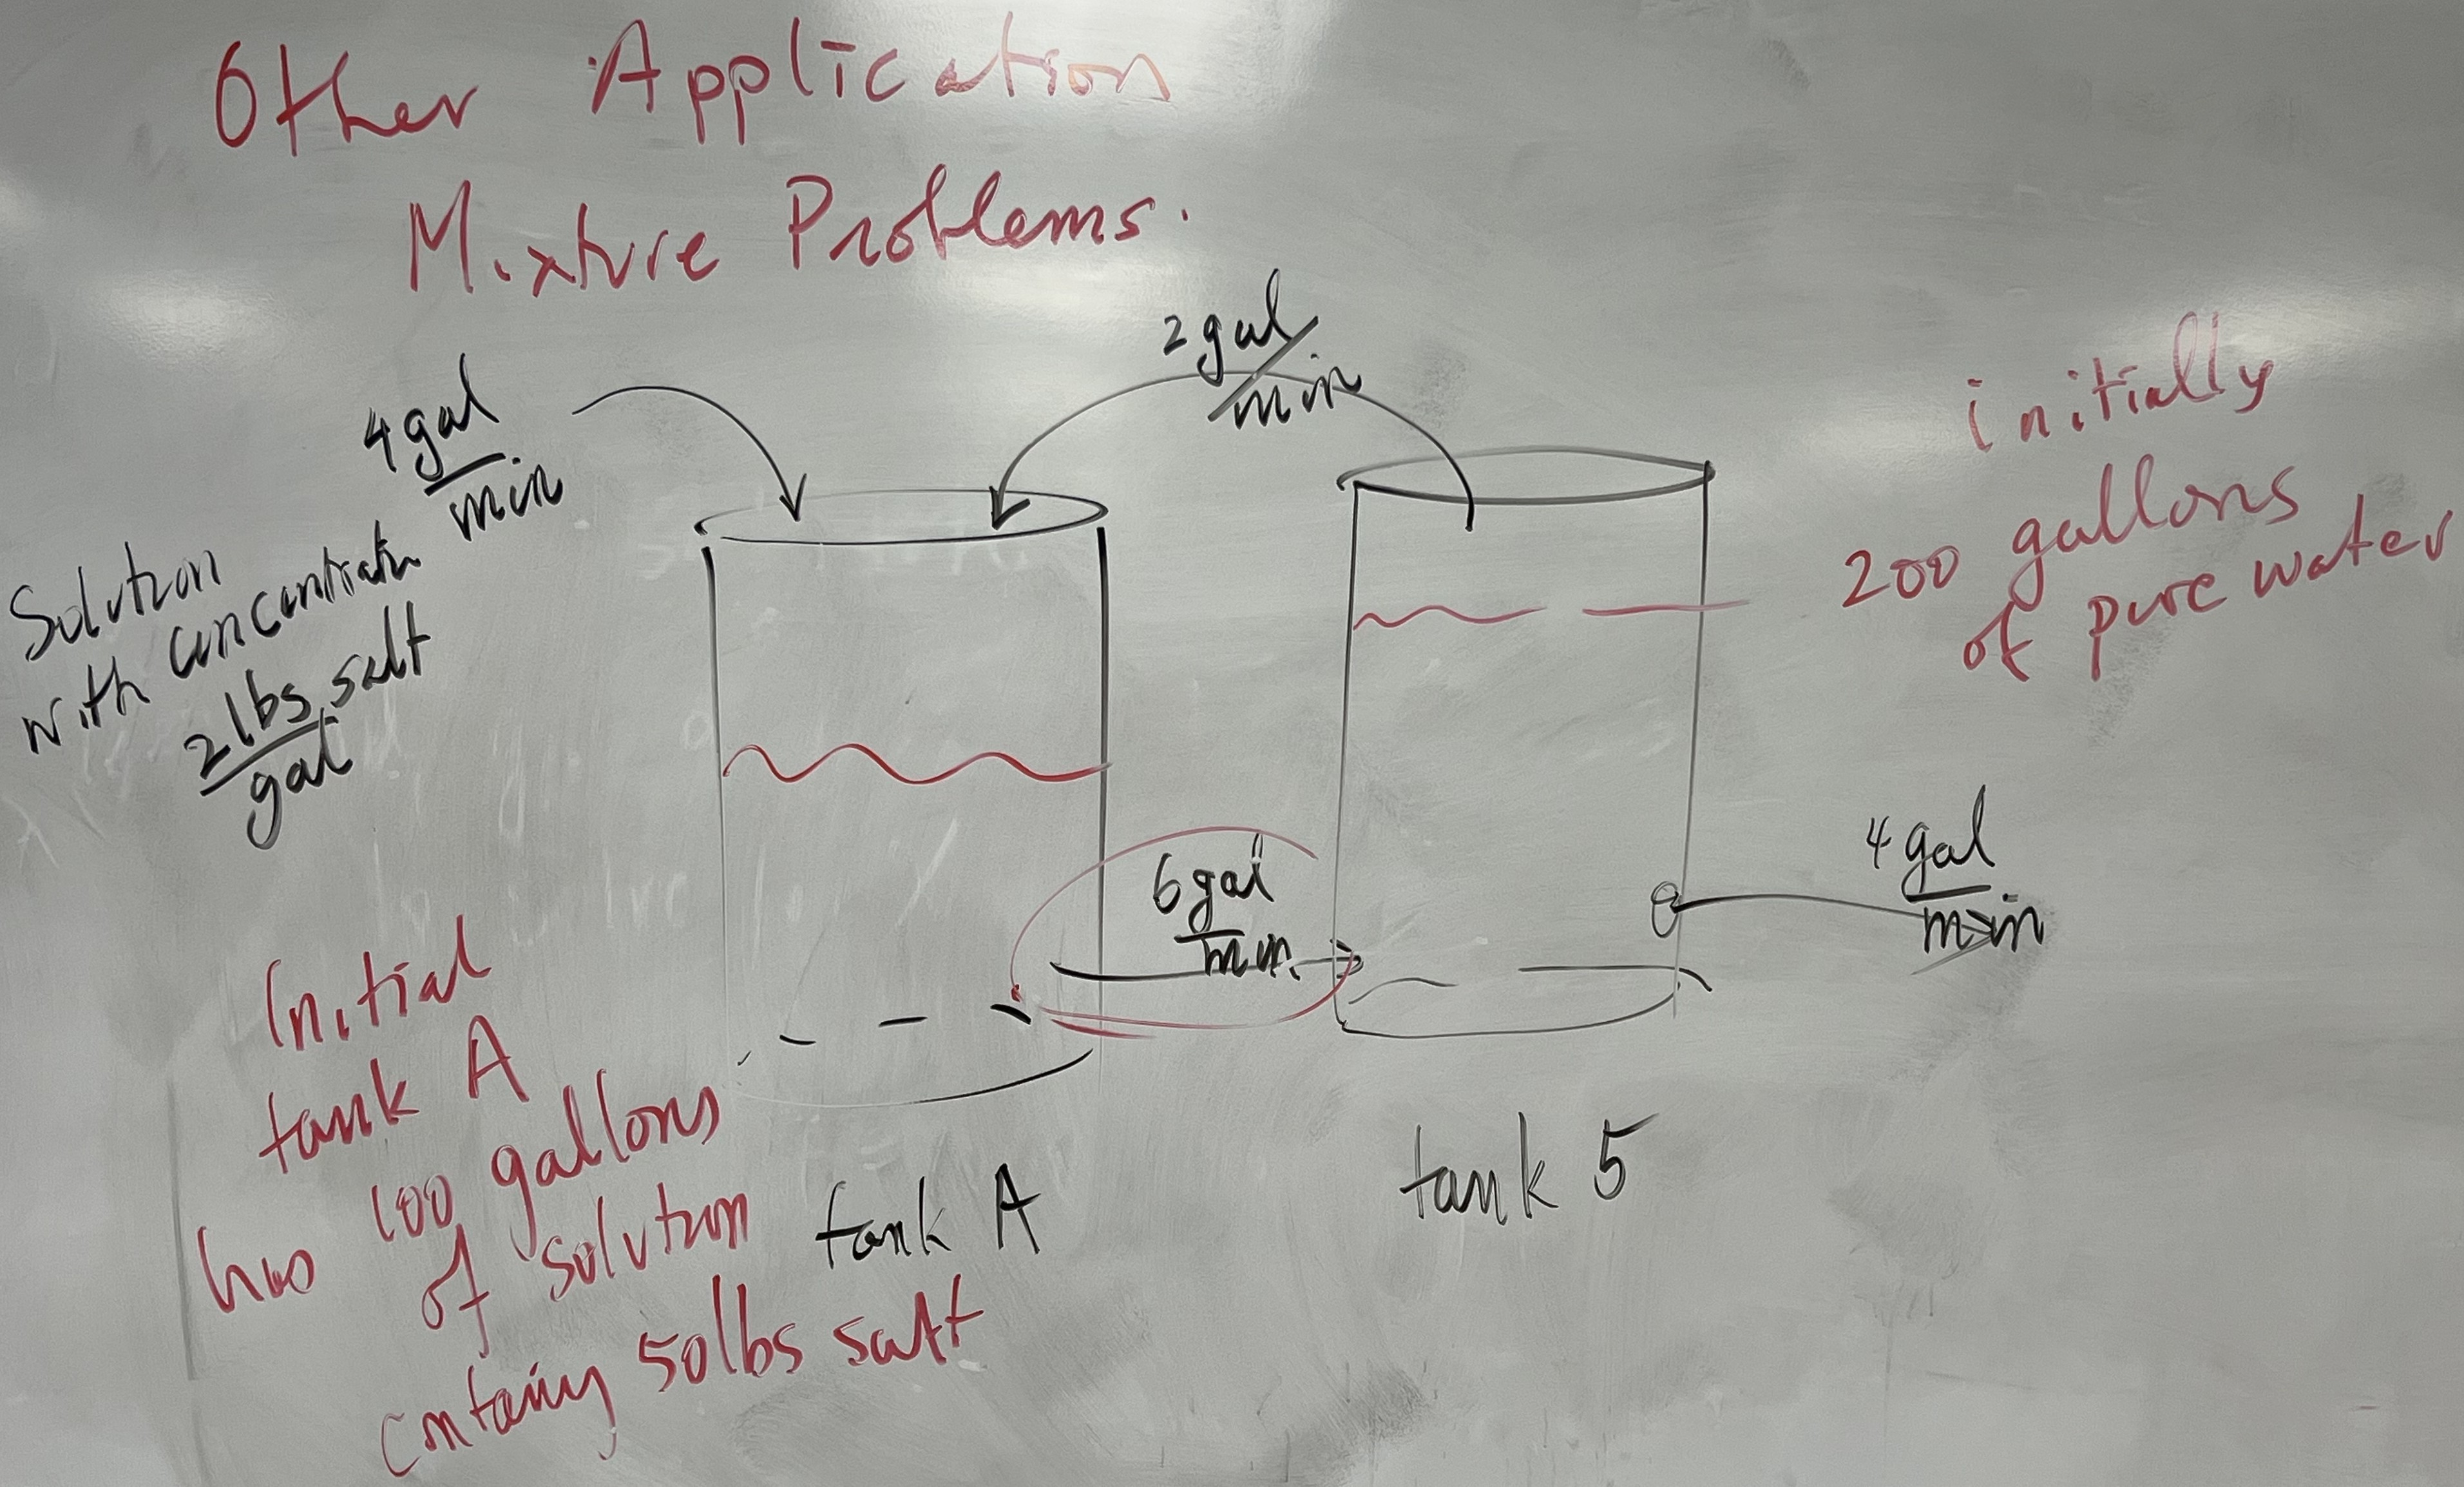
\includegraphics[width=\textwidth]{3.3_tanks}
	\caption{}
	\label{fig:3.3_tanks}
\end{figure}


Solution with concentration 2 $\frac{\mbox{lbs of salt}}{\mbox{gal}}$. Initial tank $A$ has 100 gallons of solution containing 50 lbs of salt.\\

Let $x_{1}(t)$ = \# of lbs of salt in tank $A$ at time $t$.

Let $x_{2}(t)$ = \# of lbs of salt in tank $B$ at time $t$.

Tank $A$ will always have 100 gallons of solution (6 gallons in = 6 gallons out)
some for tank $B$ with $V=200$ gal

\begin{equation*}
\begin{aligned}
	\frac{dx_{1}}{dt} &= \mbox{rate salt in to tank } A - \mbox{rate salt \textbf{out} of tank } B\\
					  &= 4\frac{gal}{min}\times2\frac{lbs}{gal} + 2\frac{gal}{min}\times\frac{\mbox{\# lbs salt in } B}{200\ gal} - \frac{6\ gal}{min}\times\frac{x_{1}}{100\ gal}\\
					  &= 8\frac{lbs}{min} + \frac{\mbox{\# lbs salt in } B}{100\ min} - \frac{3x_{1}}{50\ min}\\
					  &= 8 + \frac{x_{2}}{100} - \frac{3x_{1}}{50}\\
\end{aligned}
\end{equation*}

%</Section-3.3>

\end{document}